\documentclass{beamer}
\usepackage{config}

%Information to be included in the title page:
\title[VCS]{Usages et intérêts des sytèmes de gestion de versions (ou VCS) pour un usage professionnel et personnel}
\author{Florian Legendre}
\institute{Université de Poitiers}
\date{Année 2020 - 2021}
\logo{
\includegraphics[scale=0.1]{UP.png}}


%%% ============================================================= %%%
%%% ====================== Début des diapos ===================== %%%
%%% ============================================================= %%%

\begin{document}

\frame{\titlepage}

\begin{frame}
\frametitle{Table of Contents}
\tableofcontents
\end{frame}

%% --------------------- %%
%%        SECTION        %%
%% --------------------- %%
\AtBeginSection[]
{
  \begin{frame}
    \frametitle{Table of Contents}
    \tableofcontents[currentsection]
  \end{frame}
}
\section{La notion de version et ses implications}

% Subsection:
\subsection{Première étude de cas: notions de version/log/reset/diff}
\begin{frame}
\frametitle{Premier cas: Jean étudiant en lettres}
Jean écrit une première version de son devoir qu'il envoie à son enseignante par mail:
\begin{center}
    \includegraphics[scale=0.3]{images/firstScenario/firstScenario_diapo1.png}
\end{center}
\end{frame}

\begin{frame}
\frametitle{Premier cas: Jean étudiant en lettres}
L'enseignante de Jean suggère dans sa réponse des corrections dont Jean tient compte. Il écrit donc dans le document les corrections:
\begin{center}
    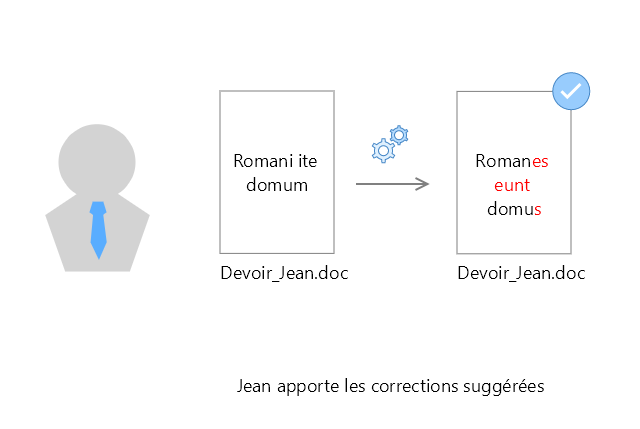
\includegraphics[scale=0.3]{images/firstScenario/firstScenario_diapo2.png}
\end{center}
\end{frame}

\begin{frame}
\frametitle{Premier cas: Jean étudiant en lettres}
Finalement, l'enseignante de Jean est allée un peu trop vite et dit à Jean qu'elle s'était trompée dans son précédent mail... Jean doit revenir à la première version en se souvenant de toutes les modifications qu'il a pu faire:
\begin{center}
    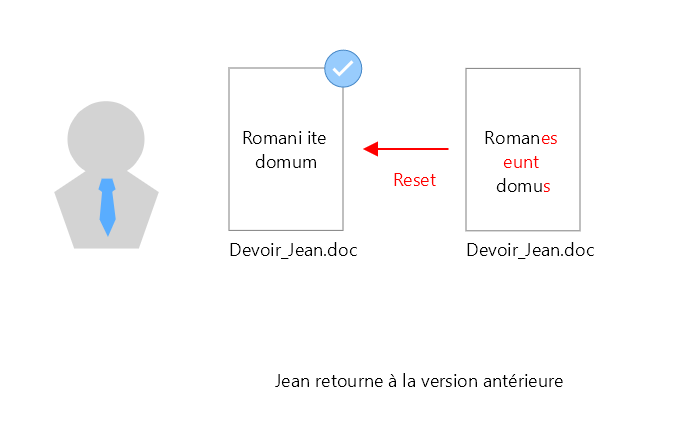
\includegraphics[scale=0.3]{images/firstScenario/firstScenario_diapo3.png}
\end{center}
\end{frame}

\begin{frame}
\frametitle{Premier cas: Jean étudiant en lettres}
Si Jean avait été un étudiant prévoyant il aurait nommé ses fichiers monDevoir\_V1 pour désigner la première version qu'il envoie à son enseignante et monDevoir\_V2 pour désigner la version tenant compte des corrections de son enseignante:
\begin{center}
    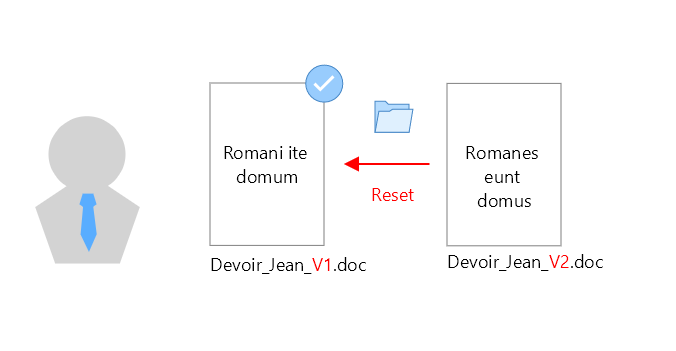
\includegraphics[scale=0.3]{images/firstScenario/firstScenario_diapo4.png}
\end{center}
\end{frame}

\begin{frame}
\frametitle{Résumé du premier cas}

Jean envoie sa version à son enseignante:
\begin{center}
    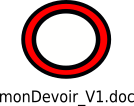
\includegraphics[scale=0.4]{images/firstScenario/firstScenario_branch2.png}
\end{center}

Jean écrit une nouvelle version tenant compte des corrections de son enseignante:
\begin{center}
    
\includegraphics[scale=0.4]{images/firstScenario/firstScenario_branch1.png}
\end{center}

Jean revient à la première version sous les conseils de son enseignante:
\begin{center}
    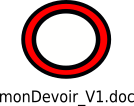
\includegraphics[scale=0.4]{images/firstScenario/firstScenario_branch2.png}
\end{center}
\end{frame}

\begin{frame}
\frametitle{Conclusion du premier cas}
Quelques notions:
\begin{itemize}
    \item \textbf{Une version:} un état d'un document à un point de sauvegarde (ou "commit") donné
    \item \textbf{Historique des versions:} fichier contenant toutes les versions passées et présente d'un document
    \item \textbf{Comparaison des versions:} Jean ne peut pas le faire facilement (à moins de lire les différentes versions) mais nous verrons que les VCS permettent de comparer les versions de l'historique entre elles en fournissant de nombreuses informations sur celles-ci (zones qui ont été supprimées ou ajoutées, etc.)
\end{itemize}
\end{frame}


% Subsection:
\subsection{Seconde étude de cas: notions de branches/merge}
\begin{frame}
\frametitle{Second cas: Jean bidouille son commentaire de texte}
On reprend depuis le début, Jean rédige un commentaire de texte, il envoie une première version à son enseignante qui la valide:
\begin{center}
    \includegraphics[scale=0.4]{images/secondScenario/firstScenario_diapo1.png}
\end{center}
\end{frame}

\begin{frame}
\frametitle{Second cas: Jean bidouille son commentaire de texte}
Bien que sa première version soit validée Jean aimerait la perfectionner... Il crée alors une "branche alternative" à son devoir:
\begin{center}
    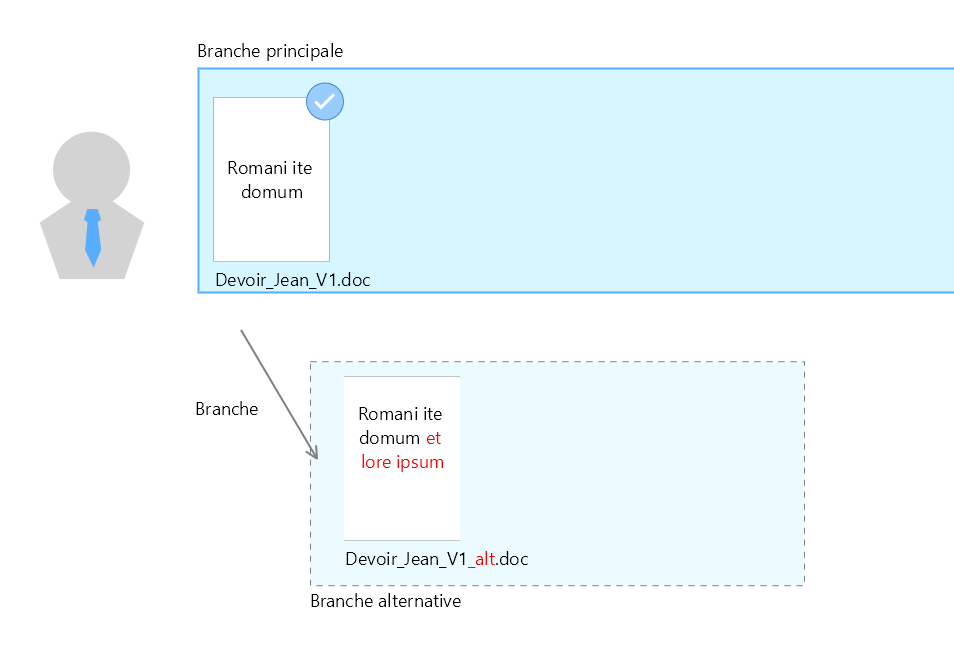
\includegraphics[scale=0.25]{images/secondScenario/secondScenario_diapo1.png}
\end{center}
\end{frame}

\begin{frame}
\frametitle{Second cas: Jean bidouille son commentaire de texte}
Juste avant d'envoyer sa version alternative, Jean se rend compte qu'il peut encore améliorer cette version en ajoutant une image de Jules César. Sauf que si l'enseignante lui dit que l'image est de trop il aimerait pouvoir revenir en arrière:
\begin{center}
    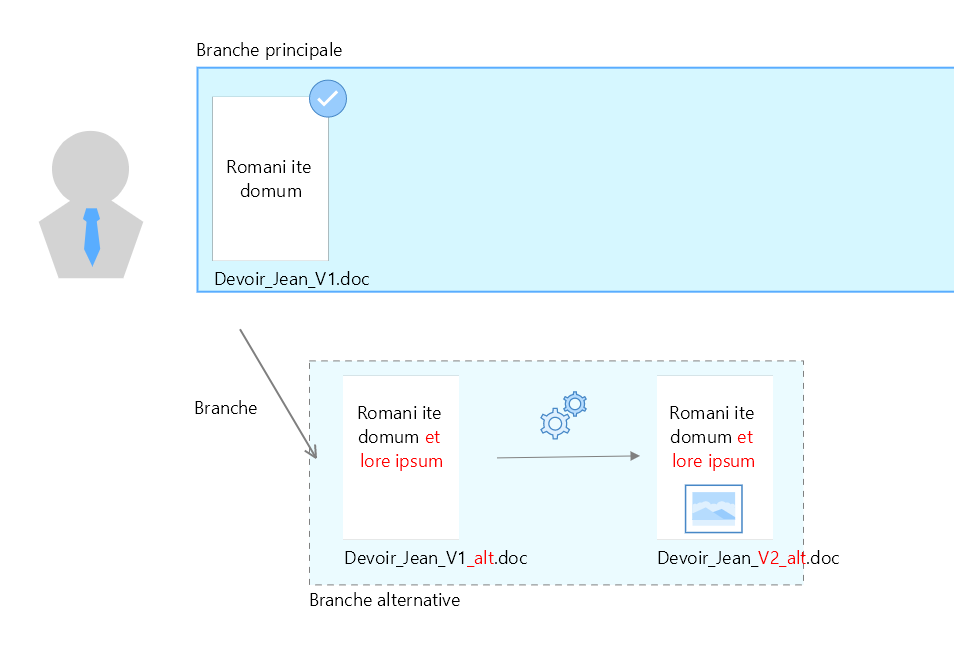
\includegraphics[scale=0.25]{images/secondScenario/secondScenario_diapo2.png}
\end{center}
\end{frame}

\begin{frame}
\frametitle{Second cas: Jean bidouille son commentaire de texte}
Jean a envoyé sa version alternative... En attendant une réponse de son enseignante il continue d'écrire son devoir dans la version qui a été validée:
\begin{center}
    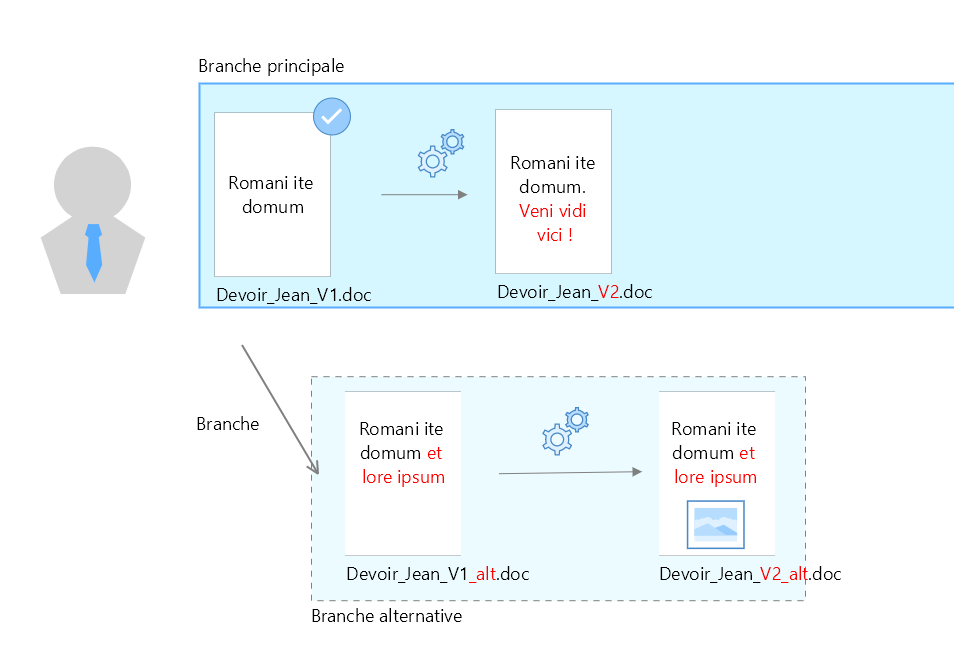
\includegraphics[scale=0.25]{images/secondScenario/secondScenario_diapo3.png}
\end{center}
\end{frame}

\begin{frame}
\frametitle{Second cas: Jean bidouille son commentaire de texte}
Jean a reçu une réponse, l'enseignante adore la nouvelle version! Jean fusionne alors ses changements avec la branche en cours:
\begin{center}
    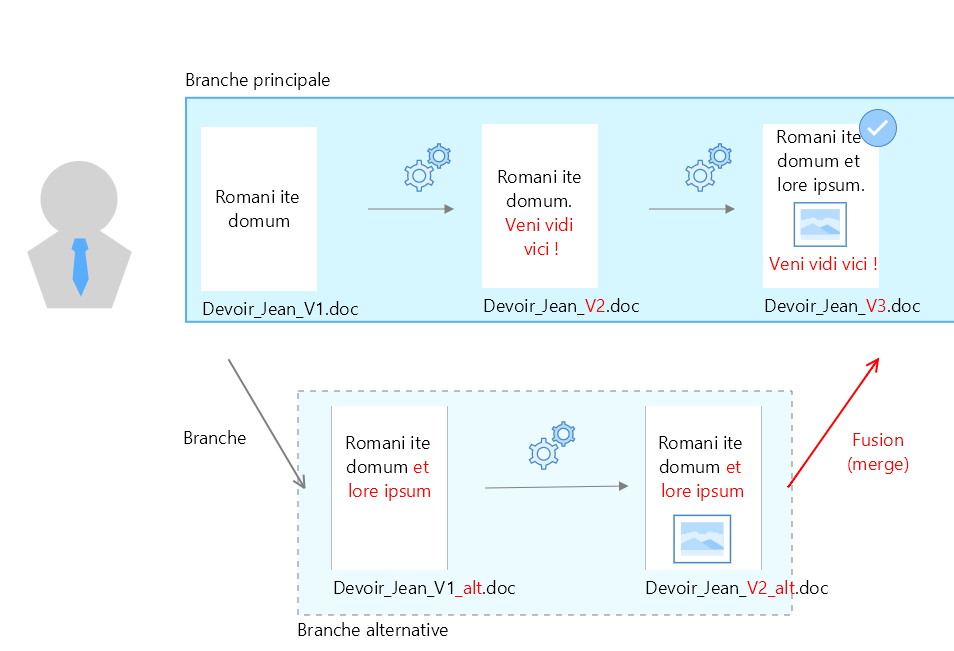
\includegraphics[scale=0.25]{images/secondScenario/secondScenario_diapo4.png}
\end{center}
\end{frame}

\begin{frame}
\frametitle{Résumé du second cas}
Si on schématise le flux des versions ("workflow") du travail de Jean on obtient le schéma suivant:

\begin{center}
    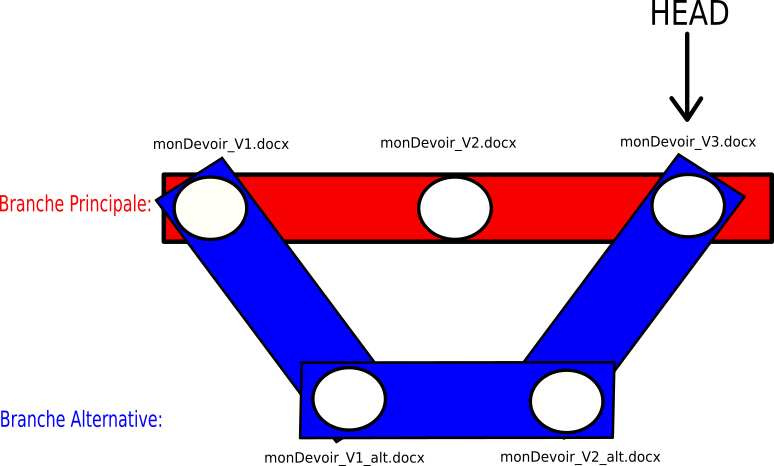
\includegraphics[scale=0.4]{images/secondScenario/secondScenario_branches.png}
\end{center}
\end{frame}

\begin{frame}
\frametitle{Remarque avant de conclure}
Vous remarquerez sur le schéma précédent un pointeur appelé "HEAD". Ce pointeur indique la version courante dans laquelle se trouve le projet de Jean.\\
\medskip

Je l'ai représenté ici pour illustrer où en était Jean à la fin de notre exemple. Mais nous verrons que Git offre des fonctionnalités pour manipuler ce pointeur (comme la commande "git checkout"...)\\
\end{frame}

\begin{frame}
\frametitle{Conclusion du second cas}
Deux nouvelles notions:
\begin{itemize}
    \item \textbf{Une branche:} une séquence de versions prenant racine dans une version donnée.
    \item \textbf{Une fusion (ou merge) de branches:} Modification d'une version d'une branche en fonction des modifications apportées à une version d'une autre branche (\textbf{ce qui inclut aussi les suppressions!})
\end{itemize}
\bigskip

\underline{Remarque:} avec un système de gestion des versions comme Git on peut donner des noms à nos branches pour les identifier et passer d'une branche à une autre aisément!
\end{frame}


% Subsection:
\subsection{Dernière étude de cas: notions de conflits/pull/push}
\begin{frame}
\frametitle{Dernier cas: Jean travaille avec Anne}
Au début tout va bien. Jean et Anne ont le même document. Pour se partager le devoir ils ont un serveur type "dropbox" où ils mettent la dernière version commune du devoir:
\begin{center}
    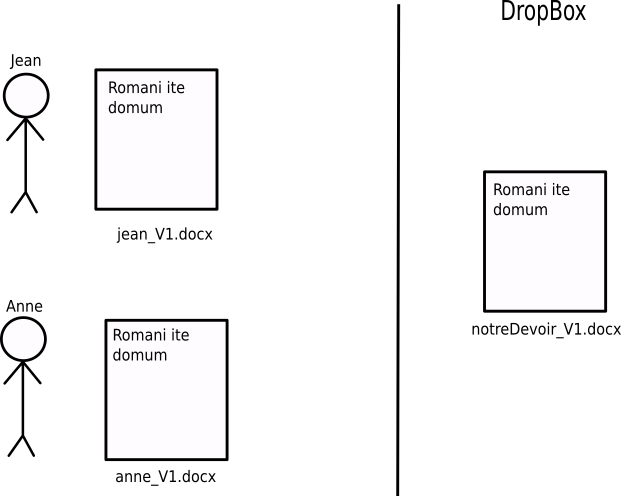
\includegraphics[scale=0.4]{images/lastScenario/lastScenario_init.png}
\end{center}
\end{frame}

\begin{frame}
\frametitle{Dernier cas: Jean travaille avec Anne}
Jean et Anne se sont bien partagé les tâches... Mais à un moment donné Jean a besoin de modifier une partie "commune". Il pense qu'Anne n'aura pas besoin de la modifier... Sauf qu'Anne pense la même chose de son côté:
\begin{center}
    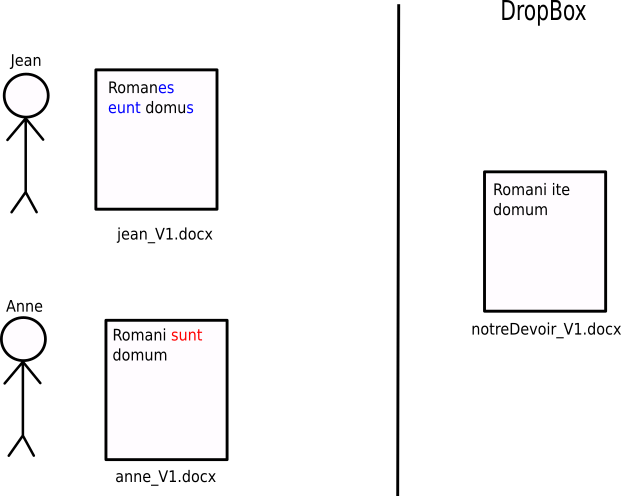
\includegraphics[scale=0.4]{images/lastScenario/lastScenario_conflict1.png}
\end{center}
\end{frame}

\begin{frame}
\frametitle{Dernier cas: Jean travaille avec Anne}
Jean met alors à jour la version commune:
\begin{center}
    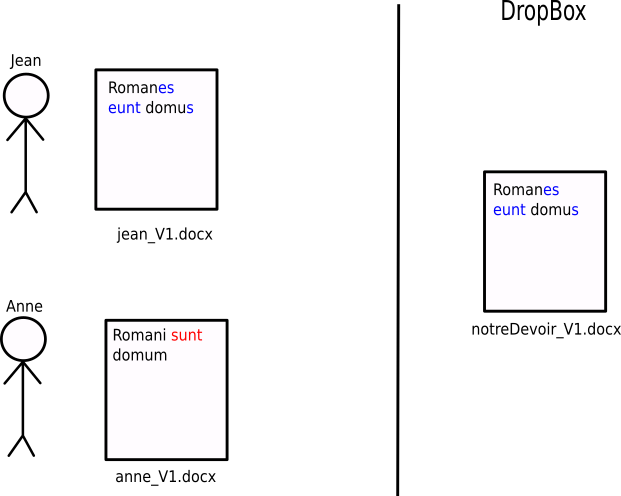
\includegraphics[scale=0.4]{images/lastScenario/lastScenario_conflict2.png}
\end{center}
\end{frame}

\begin{frame}
Puis c'est au tour d'Anne:
\frametitle{Dernier cas: Jean travaille avec Anne}
\begin{center}
    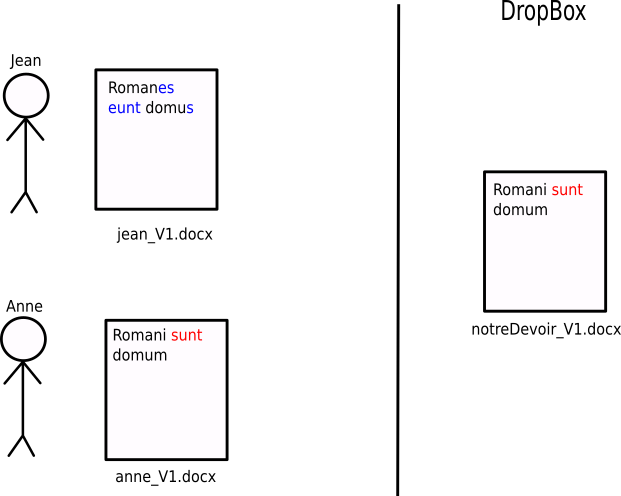
\includegraphics[scale=0.4]{images/lastScenario/lastScenario_conflict3.png}
\end{center}
\end{frame}

\begin{frame}{Dernier cas: Jean travaille avec Anne}
On comprend alors que de nombreux problèmes peuvent survenir après cette situation:
\medskip
\begin{enumerate}
    \item Si Jean ne se rend pas compte du problème suffisamment tôt ses modifications seront perdues.
    \item S'il se rend compte du problème il devra de toute façon relire toutes les parties "communes" qu'ils ont tous les deux modifiés pour revenir sur un document "propre".
    \item Si le nombre de conflits est conséquent un retour à un document "propre" peut devenir tout simplement impossible...
\end{enumerate}
\medskip
Comment Anne et Jean auraient-ils alors pu prévenir ce problème?
\end{frame}

\begin{frame}{Dernier cas: Jean travaille avec Anne}
\begin{center}
    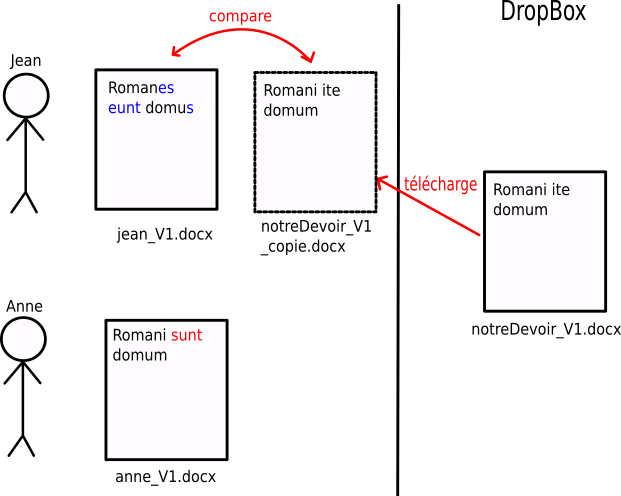
\includegraphics[scale=0.4]{images/lastScenario/lastScenario_pullpush1.png}
\end{center}
\end{frame}

\begin{frame}{Dernier cas: Jean travaille avec Anne}
\begin{center}
    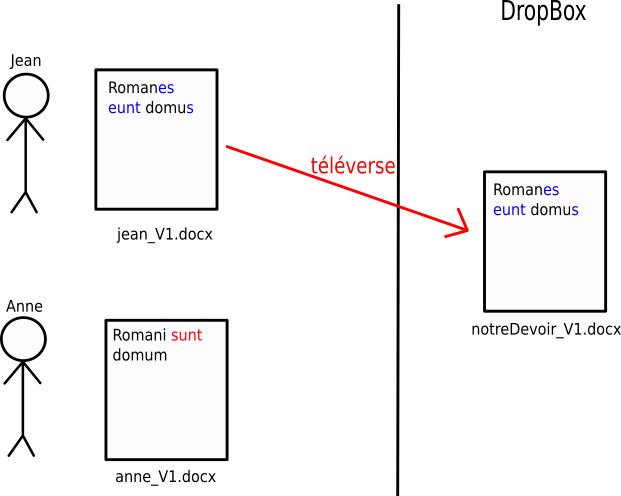
\includegraphics[scale=0.4]{images/lastScenario/lastScenario_pullpush2.png}
\end{center}
\end{frame}

\begin{frame}{Dernier cas: Jean travaille avec Anne}
\begin{center}
    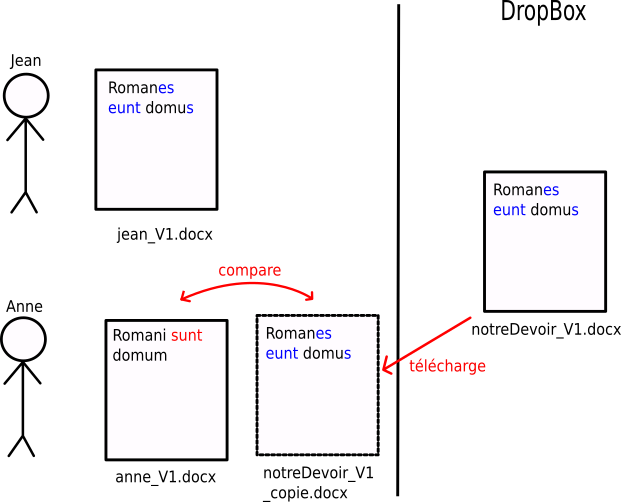
\includegraphics[scale=0.4]{images/lastScenario/lastScenario_pullpush3.png}
\end{center}
\end{frame}

\begin{frame}
\frametitle{Résumé du dernier cas}
\begin{itemize}
    \item \textbf{Un conflit} survient lorsque deux collaborateurs sur un même document éditent la même zone de ce document.
    \item Une manière de gérer ce conflit est de vérifier que le document distant n'a pas été modifié avant de le mettre à jour. Ce processus se fait en deux étape: 1) on télécharge le document (cf. "fetch") 2) on compare/fusionne les documents si besoin. Sous Git, ces deux opérations combinées s'appellent un "\textbf{pull}". 
    \item Une fois que ce "pull" a été fait on peut alors mettre à jour le document distant. Ce processus de téléversement (ou "upload") est appelé sous Git un "\textbf{push}".
\end{itemize}
\end{frame}

\begin{frame}
\frametitle{Conclusion du dernier cas}
La gestion "à la main" des conflits et des mises à jour d'un document peut être sérieusement laborieuse à mesure que le projet grandit.
\medskip

Ajouté à cela la notion de branches à gérer, voire de branches sur le document distant (et/ou sur le document local) et le tout devient au mieux très chronophage, au pire menace le développement futur du projet.
\medskip
\end{frame}


%% --------------------- %%
%%        SECTION        %%
%% --------------------- %%
\AtBeginSection[]
{
  \begin{frame}
    \frametitle{Table of Contents}
    \tableofcontents[currentsection]
  \end{frame}
}
\section{Les VCS et Git}

% Subsection:
\subsection{Les services offerts par les VCS}
\begin{frame}
\frametitle{Ingéniérie logicielle = VCS}

Les VCS ("Version Control System") offrent généralement les services suivants:
\medskip

\begin{enumerate}
    \item Sauvegarde de versions
    \item Historique de versions 
    \item Comparaison de versions
    \item Branches de versions
    \item Partage de versions
    \item Identification de conflits
\end{enumerate}
\medskip

\underline{Remarque:} Tout peut être versionné!
\end{frame}

% Subsection:
\subsection{Les VCS comparés aux outils collaboratifs en ligne}
\begin{frame}
\frametitle{VCS versus Google Docs}
\begin{tabular}{ | m{12em} | m{12em} | }
    \hline
    
    \textbf{VCS} & \textbf{Google Docs}\\
        
    \hline
    
    \begin{enumerate}
    \item Sauvegarde de versions
    \item Historique de versions 
    \item Comparaison de versions
    \item Branches de versions
    \item Partage de versions
    \item Identification de conflits
    \end{enumerate}
    
    & 
    
    \begin{enumerate}
    \item Sauvegarde de versions
    \item Historique de versions
    \item Comparaison de versions
    \end{enumerate} \\
    
    \hline
\end{tabular}
\medskip

\underline{Remarque:} On ne peut pas exécuter du code dans google docs non plus...
\end{frame}

% Subsection:
\subsection{Les services offerts par Git}
\begin{frame}
\frametitle{Git: un VCS distribué, gratuit et open-source}
Les VCS locaux:
\begin{center}
    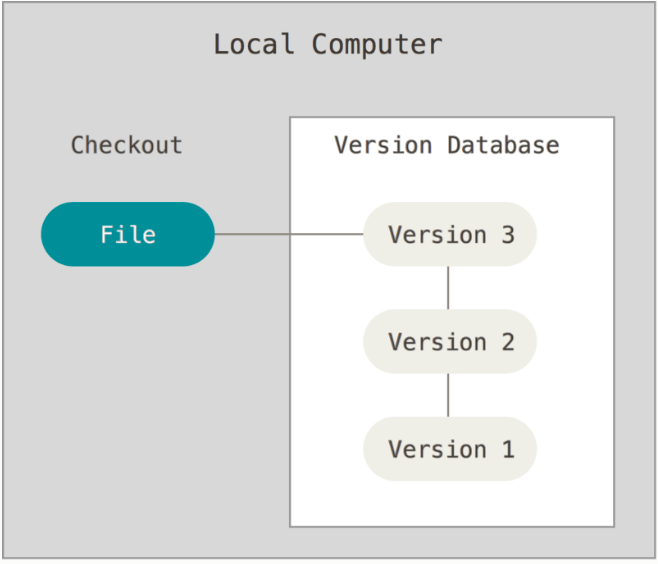
\includegraphics[scale=0.25]{images/vcs/vcs_local.png}
\end{center}

\underline{Remarque:} Checkout indique ici que le projet "File" est\\
\smallskip
dans l'état correspondant à la "Version 3"
\end{frame}

\begin{frame}
\frametitle{Git: un VCS distribué, gratuit et open-source}
Les VCS centralisés:
\begin{center}
    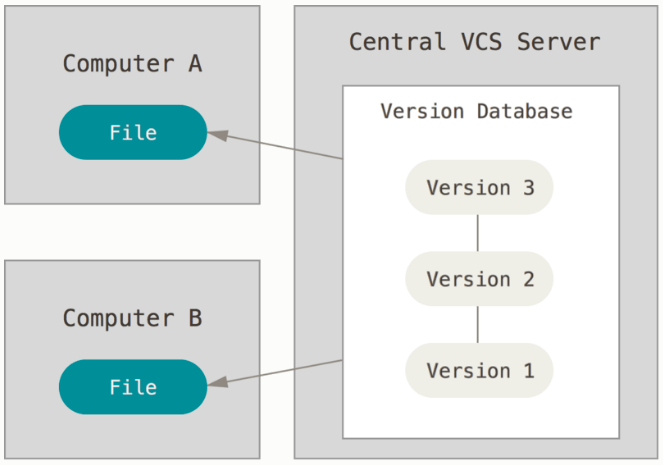
\includegraphics[scale=0.25]{images/vcs/vcs_centralized.png}
\end{center}
\end{frame}

\begin{frame}
\frametitle{Git: un VCS distribué, gratuit et open-source}
Les VCS distribués:
\begin{center}
    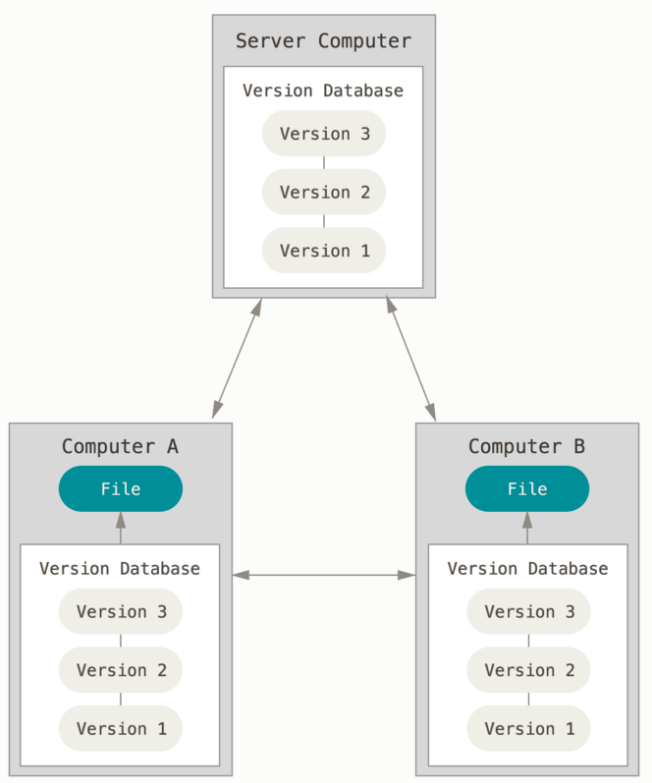
\includegraphics[scale=0.25]{images/vcs/vcs_distributed.png}
\end{center}
\end{frame}

\begin{frame}
\frametitle{Git: un VCS distribué, gratuit et open-source}
Les avantages des VCS distribués:
\begin{enumerate}
    \item Si on n'a pas de connexion internet on peut continuer à travailler
    \item Si le serveur central est défaillant quelqu'un aura l'historique
    \item On peut facilement changer de dépôt distant "de référence" (cf. les "fork")
\end{enumerate}
\end{frame}

\begin{frame}
\frametitle{Git: un VCS distribué, gratuit et open-source}
\begin{tabular}{ | m{12em} | m{12em} | }
    \hline
    
    \textbf{VCS centralisés} & \textbf{VCS distribués}\\
        
    \hline
    
    \begin{itemize}
    \item SVN
    \end{itemize}
    
    & 
    
    \begin{itemize}
    \item Git
    \item Mercurial
    \item Bazaar
    \end{itemize} \\
    
    \hline
\end{tabular}
\end{frame}


% Subsection:
\subsection{Les services offerts par GitHub}
\begin{frame}
\frametitle{Git n'est pas GitHub et réciproquement}
\begin{tabular}{ | m{13em} | m{13em} | }
    \hline
    
    \textbf{Git} & \textbf{GitHub}\\
        
    \hline
    
    \begin{enumerate}
        \item Git est un VCS
        \item Git a une fonctionnalité cliente lui permettant de communiquer avec un dépôt
        \item Git a été écrit par Linus Torvald (l'auteur du noyau Linux)
        \item Les compétiteurs de Git sont Mercury, Bazaar, SVN...
    \end{enumerate}
    & 
    
    \begin{enumerate}
    \item GitHub est l'équivalent de DropBox avec des fonctionnalités spécialisées pour les VCS
    \item GitHub est un serveur web d'hébergement (aussi appelé "dépôt")
    \item GitHub appartient à Microsoft
    \item Les compétiteurs de GitHub sont GitLab, GitBucket...
    \end{enumerate} \\
    
    \hline
\end{tabular}

\end{frame}


%% --------------------- %%
%%        SECTION        %%
%% --------------------- %%
\AtBeginSection[]
{
  \begin{frame}
    \frametitle{Table of Contents}
    \tableofcontents[currentsection]
  \end{frame}
}
\section{Le plan de la formation}

\begin{frame}{Le flot de commande Git}
\begin{center}
    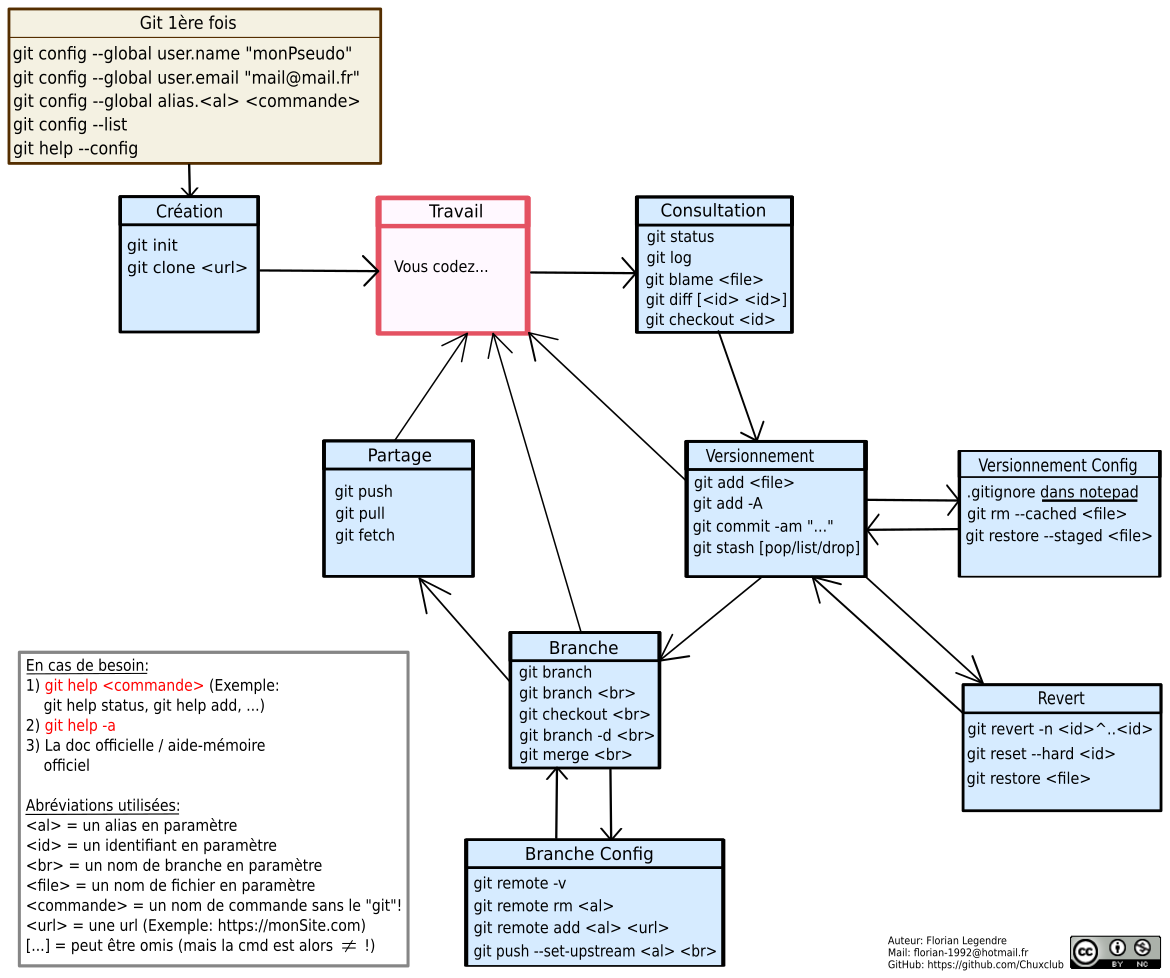
\includegraphics[scale=0.28]{images/gitCommandFlow/gitCommandFlow.png}
\end{center}
\end{frame}

\begin{frame}{La boucle locale mono-branche}
\begin{center}
    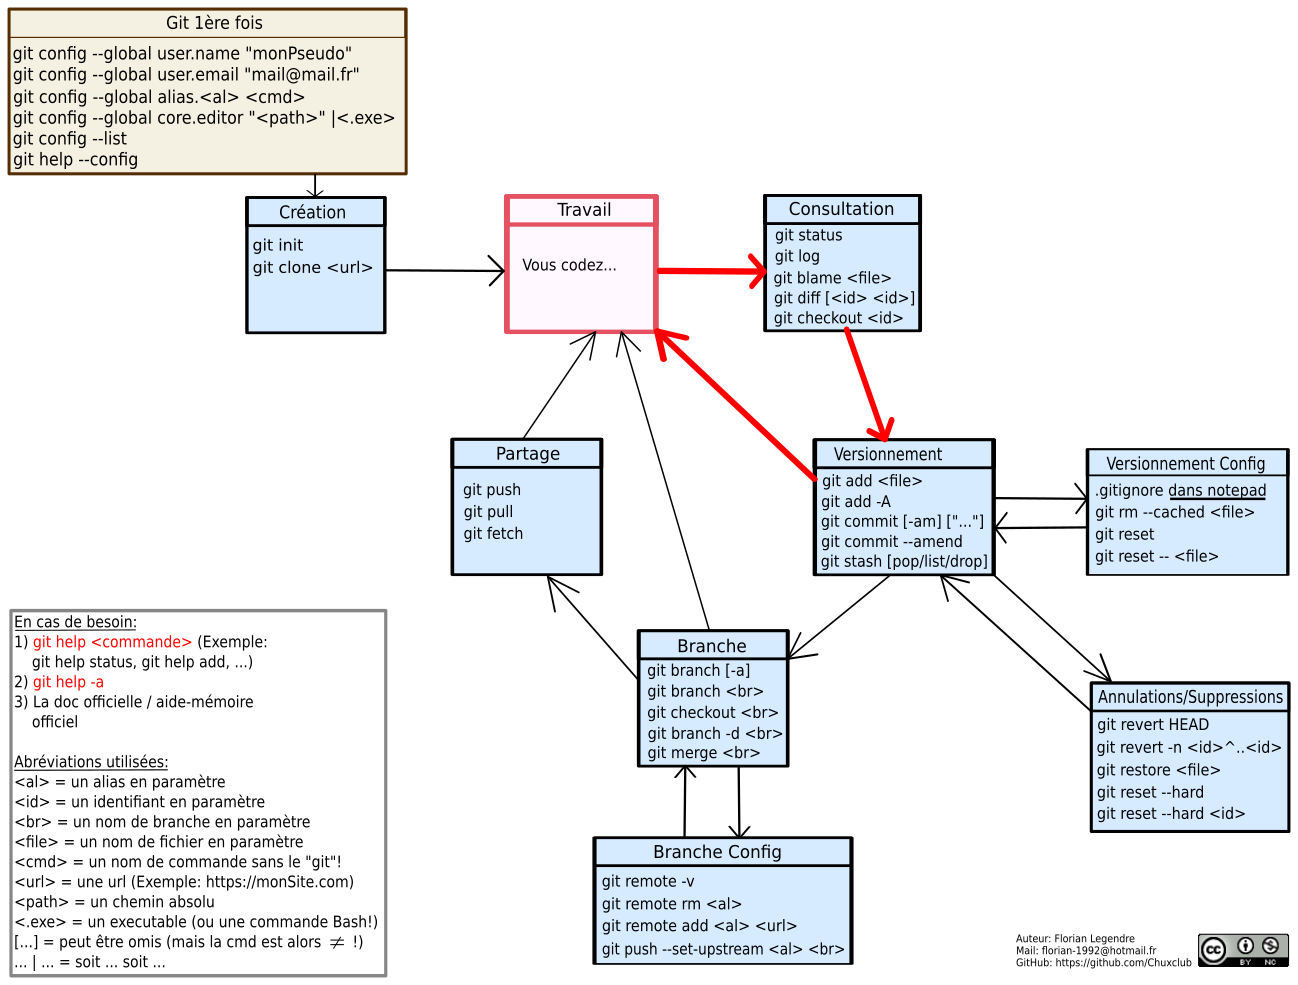
\includegraphics[scale=0.28]{images/gitCommandFlow/gitCommandFlow_localLoop.png}
\end{center}
\end{frame}

\begin{frame}{La boucle locale multibranche}
\begin{center}
    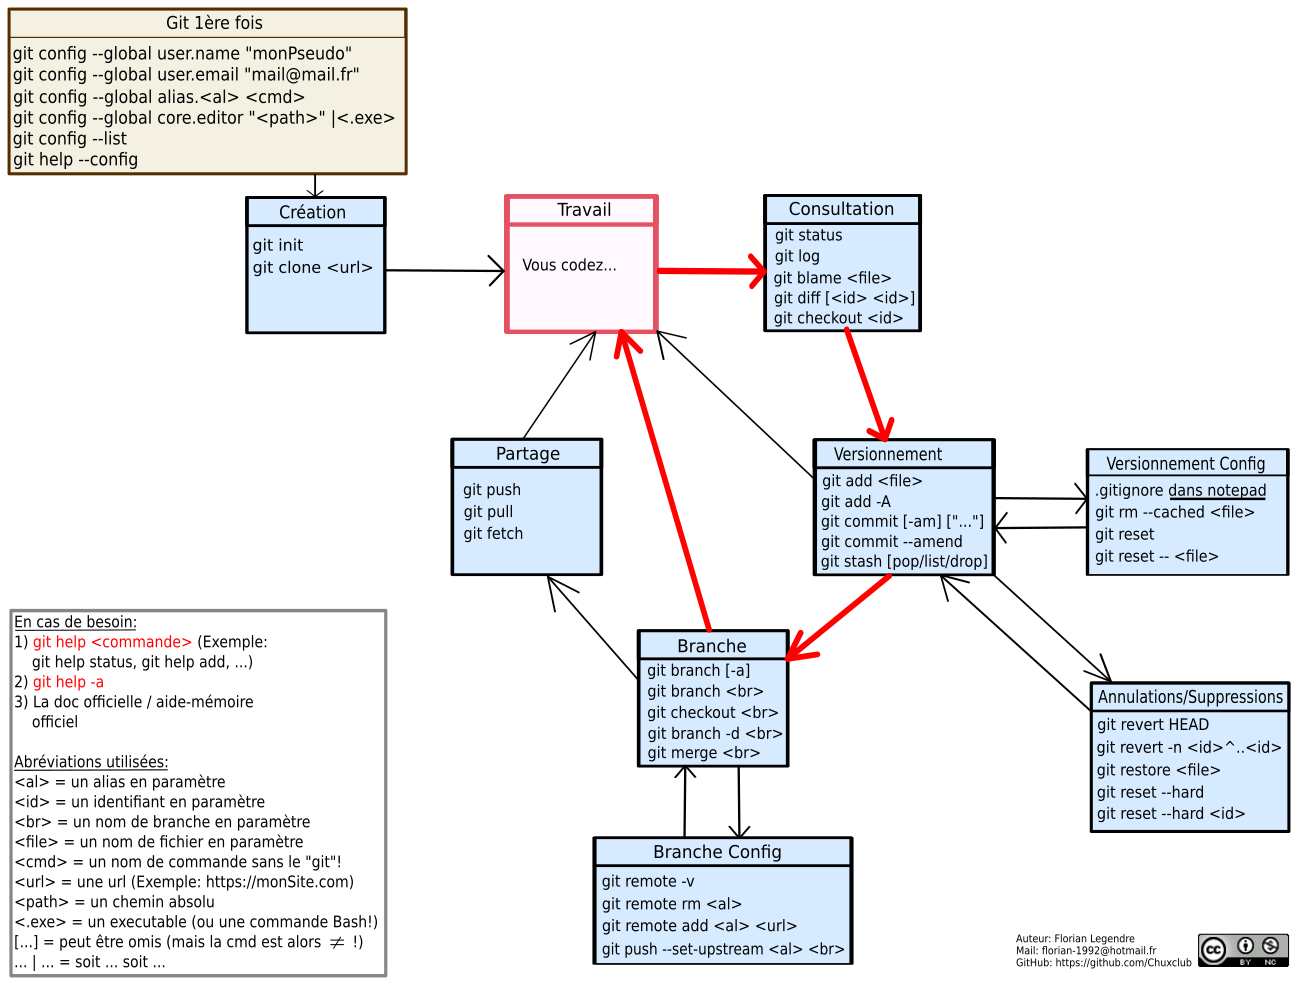
\includegraphics[scale=0.28]{images/gitCommandFlow/gitCommandFlow_multilocalLoop.png}
\end{center}
\end{frame}

\begin{frame}{Git collaboratif}
\begin{center}
    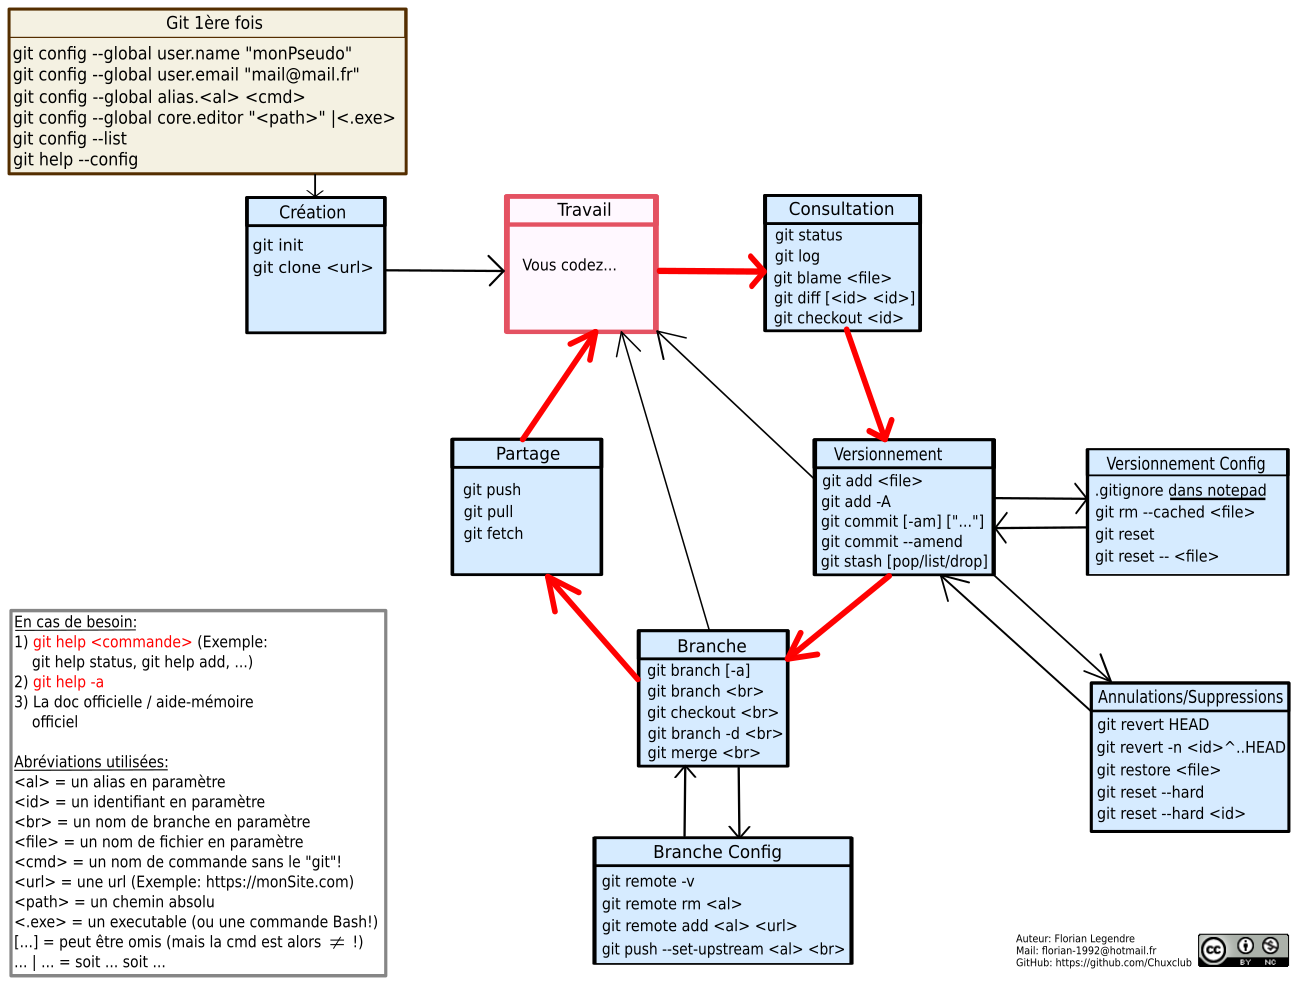
\includegraphics[scale=0.28]{images/gitCommandFlow/gitCommandFlow_connectedLoop.png}
\end{center}
\end{frame}

\end{document}
